\documentclass[12pt]{article}

\usepackage{a4wide, amsfonts, epsfig}

\begin{document}
\begin{center}
{\bf EMAT10001 Workshop Sheet 17 outline solutions.}\\[1cm]{} Conor Houghton 2014-02-26
\end{center}

\subsubsection*{Work sheet}

\begin{enumerate}

\item Establish that
\begin{equation}
\int^\pi_{-\pi}~dt~ \sin mt ~\cos nt=0
\end{equation}
for integers $n$ and $m$.

\textbf{Solution: } This is an exercise in trigonometry and uses first the trignometric identity
\begin{equation}
\int^\pi_{-\pi}~dt~ \sin mt ~\cos nt=\frac{1}{2}\int^\pi_{-\pi}~dt~ [\sin{(n-m)t}-\sin{(n+m)t)}]=0
\end{equation}
and then the fact that the integral of a trignometric function over its whole period is zero. This fact is used a lot; take sine for example, and let $N$ be an integer. Consider
\begin{equation}
I=\int_{-\pi}^\pi {\sin{Nt}}dt
\end{equation}
Let $s=Nt$ so $ds=Ndt$ and when $t=\pi$ then $s=N\pi$ and $t=-\pi$ then $s=-N\pi$. Hence
\begin{equation}
I=\frac{1}{N}\int_{-N\pi}^{N\pi} {\sin{t}}dt
\end{equation}
and then, if $N$ is an integer, periodicity gives
\begin{equation}
I=\int_{-\pi}^{\pi} {\sin{t}}dt=-\cos{\pi}+\cos{\pi}=0
\end{equation}
The exception is $n=m$ in which case the first term is just zero. 

\item What is $\sum_{n=0}^\infty a_n\delta_{n3}$?

\textbf{Solution: } The $\delta_{n3}$ is zero unless $n=3$, we are summing over all $n$, including $n=3$ so the answer is $a_3$.

\item Show by checking whether $f(t)=-f(-t)$ for odd, $f(t)=f(-t)$ for even and neither for neither which of the following are odd, even or neither: $\sin{t}$, $t^3+t$, $t^3+2t^2$ and $|t|$.

\textbf{Solutions: }: odd, odd, neither, even.


\item Consider an odd function $f(t)$. By doing a change of variable
  $t'=-t$ show 
 \begin{equation}
\int_{-1}^1f(t)dt=0
\end{equation}

\textbf{Solution: }
\begin{equation}
I=\int_{1}^{-1}f(-t')(-dt')=-\int_{1}^{-1}[-f(t')](-dt')=\int_{-1}^1f(t')dt'=-I
\end{equation}
therefore $I=-I$ so $I=0$.

\item If $f(t)$ is even and $g(t)$ is odd, what is $f(t)g(t)$?

\textbf{Solution: } Let $h(t)=f(t)g(t)$ so
$h(-t)=f(-t)g(-t)=-f(t)g(t)=-h(t)$, so odd.

\item What is the Fourier series for 
\begin{equation}
f(t)=\left\{\begin{array}{ll}-1&t\in(-\pi,-\pi/2)\\
                             1 &t\in(-\pi/2,\pi/2)\\
                             -1&t\in(\pi/2,\pi)
\end{array}\right.
\end{equation}
with $f(t+2\pi)=f(t)$. Try to use odd and even arguments to avoid
doing the integral for $b_n$.

\textbf{Solution: } So, since $f(t)$ is even and $sin{nt}$ is odd, all the integrals involve sine are zero by the arguments above, the $a_0$ is also zero because the function is one and -1 an equal amount, making its integral zero. So
\begin{equation}
a_n=\frac{1}{\pi}\int_{-\pi}^\pi f(t)\cos{nt}dt=\frac{2}{\pi}\int_0^\pi f(t)\cos{nt}dt
\end{equation}
where I have used the evenness of the integrand, what happens from
$-\pi$ to zero is the same as what happens from zero to $\pi$. Now,
putting in the value of $f(t)$
\begin{equation}
\frac{\pi}{2}a_n=\int_0^{\pi/2}\cos{nt}dt-\int_{\pi/2}^\pi\cos{nt}dt
\end{equation}
and integrating
\begin{equation}
\frac{\pi}{2}a_n=\frac{1}{n}\sin{nt}]_0^{\pi/2}-\frac{1}{n}\sin{nt}]_{\pi/2}^\pi
\end{equation}
or
\begin{equation}
\frac{2}{\pi}a_n=\frac{2}{n}\sin{n\pi/2}-\sin{n\pi}
\end{equation}
and $\sin{n\pi}=0$ for all $n$, as for $n\pi/2$, if $n=1$ this is the sine of $\pi/2$ which is one, for $n=2$ it is zero, for $n=3$ it is -1, for $n=4$ it is zero again and then it repeats, so it is zero for $n$ even and for $n$ odd it is $(-1)^{(n-1)/2}$, so
\begin{equation}
a_n=\frac{4}{n\pi}(-1)^{(n-1)/2}
\end{equation}
for $n$ odd and zero for $n$ even, giving
\begin{equation}
f(t)=\sum_{n\mbox{ odd}}\frac{4}{n\pi}(-1)^{(n-1)/2}\cos{nt}
\end{equation}


\item There are, roughly speaking, two different types of sleep, slow
  wave sleep (SWS) when the brain is largely in active and the body is
  relaxed, and rapid eye movement (REM) sleep when we dream, the brain
  has a similar activity pattern to waking and the body is
  paralysed. This was discovered using electroencephalogram (EEG), the
  recording of the electrical activity in the brain using electrodes
  placed on the scalp. Here we see, on the left, EEG traces for a
  mouse during REM, SWS and waking, on the right we see a measure of
  the size of the Fourier components, roughly the $a_n$ and $b_n$ for
  different frequencies: $\sin(n t)$ has period $2\pi/n$ and so has
  frequency $n/2\pi$. Although the brain is largely inactive during
  SWS what little activity there is is synchronized and is
  characterized by delta waves and theta waves. Can you guess what
  frequency delta waves and theta waves are at? [Picture taken from Lima SL, Rattenborg NC, Lesku JA, Amlaner CJ. (2005) \textsl{Sleeping under the risk of predation.} Animal Behaviour 70:723-736.]  
\begin{center}
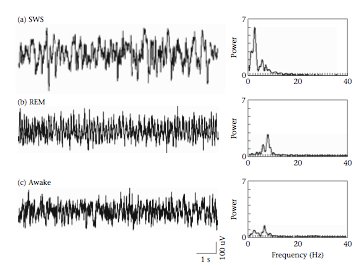
\includegraphics{SleepGeneral.png}
\end{center}

\textbf{Solution: } Long question, short answer, you can see from the graph that delta is 1-3 Hz and theta is 7-8 Hz.
\end{enumerate}

 \end{document}
